%%%%%%%%%%%%%%%%%%%%%%%%%%%%%%%%%%%%%%%%%%%%%%%%%%%%%%%%%%%%%%%%%%%%%%%%%%
\chapter{Optimalizace velikosti bajtkódu}\label{Tool}

% TODO 
% *
V této kapitole analyzuji obsah vybraného vzorku \texttt{class} souborů a na základě zjištěných poznatků navrhuji metody pro optimalizaci jejich velikosti. 

%%%%%%%%%%%%%%%%%%%%%%%%%%%%%%%%%%%%%%%%%%%%%%%%%%%%%%%%%%%%%%%%%%%%%%%%%%
\section{Analýza bajtkódu}\label{Analysis}

% Popis způsobu analýzy rozsáhlého vzorku testovacích dat, prezentace výsledků a zhodnocení.

Pomocí nástroje \texttt{jbyco} jsem získala data reprezentující vybraný vzorek testovacích souborů a tato data následně zpracovala a vyhodnotila. Zkoumala jsem velikosti položek v~\texttt{class} souborech, užití lokálních proměnných a parametrů metod a typické sekvence instrukcí. Testovací vzorek jsem vytvořila z~\texttt{jar} souborů stažených z~\texttt{http://mvnrepository.com}. Z~populárních kategorií jsem vybrala nejčastěji stahované soubory. Zvolený vzorek se skládal z 95 souborů o celkové velikosti 102,4 MB a obsahoval 59 230 \texttt{class} souborů.

\subsubsection{Velikost položek v souboru}

Typický \texttt{class} soubor z velkého vzorku obsahuje v průměru 117 konstant v tabulce konstant, 2 členské proměnné, 8 metod, 163 instrukcí a 29 atributů. Ze zkoumání celkové velikosti těchto položek vyplynulo, že konstanty tvoří 64\% z celkové velikosti všech souborů, členské proměnné 1\%, metody 2\% a instrukce 10\%.
%Součet velikostí všech atributů ku celkové velikosti souborů tvoří 47\%, ale tato hodnota je nic nevypovídající, neboť atributy mohou být součástí jiných atributů a jejich velikost je tedy započítána vícekrát. 
Nejvýznamnější atributy jsou pak \texttt{Code} s velikostí 30\%, informativní atributy s velikostí 14\% a \texttt{StackMapTable} s velikostí 2\%.

Při bližším pohledu na velikosti konstant se ukázalo, že 89\% z celkové velikosti konstant je tvořen pouze konstantami typu \textit{constant\_utf8}. Tedy konstantami popisujícími řetězce v souboru. Z těchto řetězců pak 61\% obsahuje názvy tříd, metod a členských proměnných a popisy jejich typů. Konstanty popisující číselné a řetězcové hodnoty tvoří 1\% z celkové velikosti konstant a zbývající konstanty pro popisy tříd, metod a proměnných tvoří 10\%.

Zkoumání instrukcí z hlediska jejich velikosti ukázalo, že prvních pět nejobjemnějších instrukcí tvoří 40\% z celkové velikosti instrukcí. Jsou to instrukce pro volání metod, načtení hodnoty z členské proměnné a načtení reference na objekt z lokální proměnné s indexem 0. Na této pozici se často vyskytuje reference na aktuální objekt. Z instrukcí s proměnnou délkou má instrukce \texttt{tableswitch} v průměru velikost 107 B a instrukce \texttt{lookupswitch} velikost 43 B.

% TODO tabulka celkových velikostí
% TODO tabulka řetězců
% TODO tabulka informativních atributů
% TODO tabulka nejčastějších instrukcí

\subsubsection{Užití lokálních proměnných a parametrů metody}

Data popisující užití parametrů a lokálních proměnných jsou znázorněna v grafech \ref{params} a \ref{vars}. Z dat vyplývá, že z lokálních proměnných obsahujících argumenty metody se tyto hodnoty načtou průměrně jedenkrát a dále se s nimi nepracuje. S nižším indexem proměnné počet načítání roste až k hodnotě 2,5 pro index 0. V tomto indexu se u nestatických metod předává reference na aktuální objekt (\texttt{this}). S lokálními proměnnými, které neslouží k předávání parametrů, se průměrně provádí 4,2 operací načítání, 1,8 operací vkládání a 0,3 operací inkrementace.

\begin{figure}[h!]
\centering
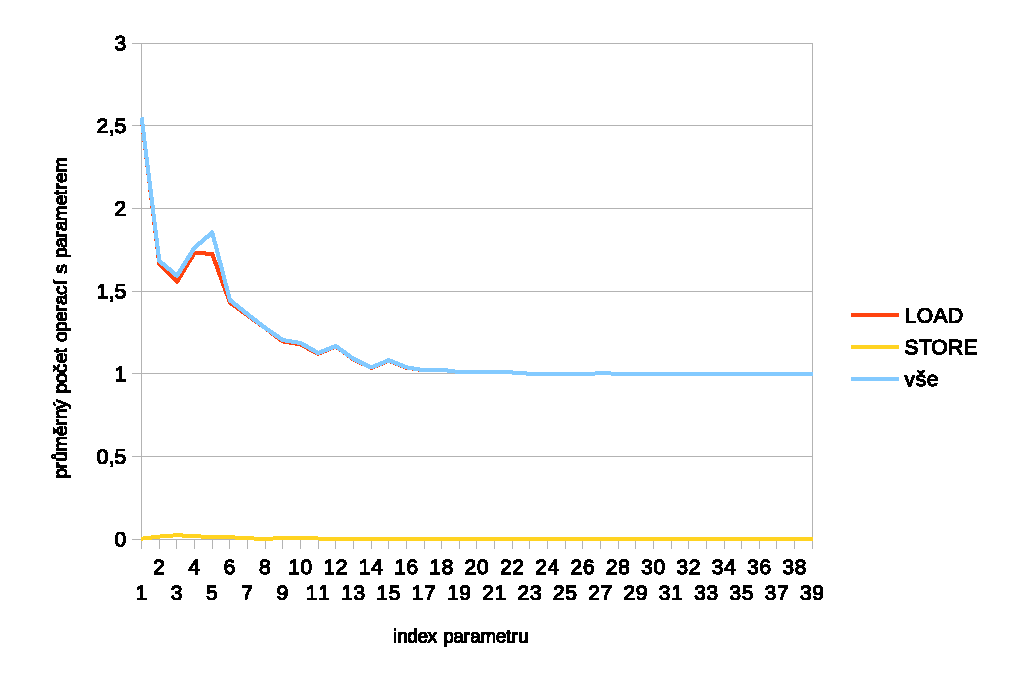
\includegraphics[scale=0.9]{fig/params}
\caption{Průměrné počty operací s parametry metod.}\label{params}
\end{figure}

\begin{figure}[h!]
\centering
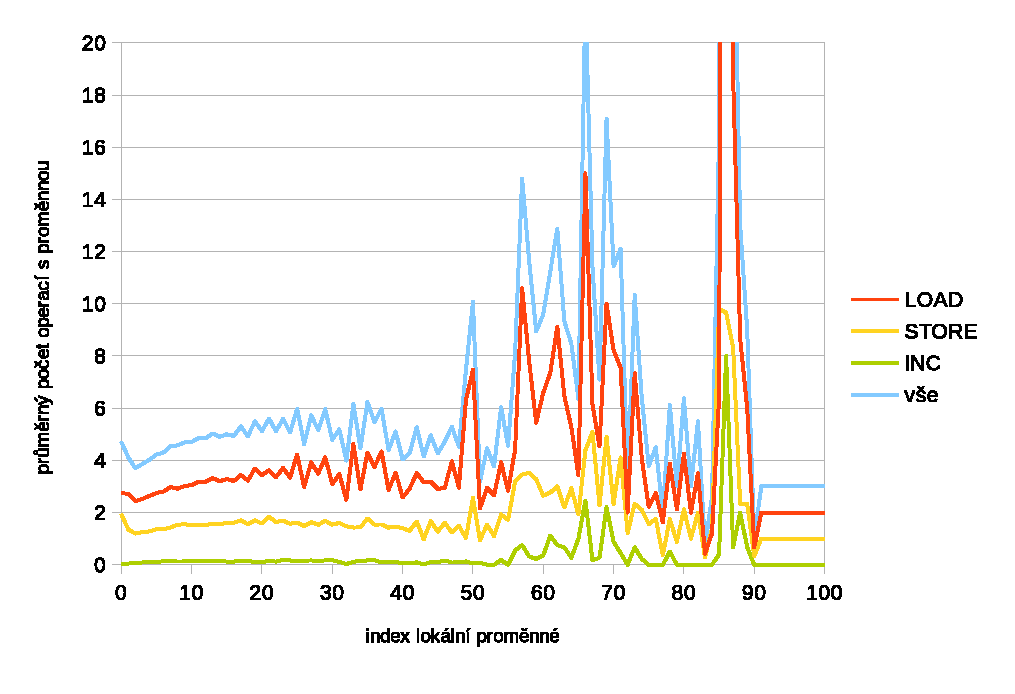
\includegraphics[scale=0.9]{fig/locals} 
\caption{Průměrné počty operací s lokálními proměnnými.}\label{vars}
\end{figure}

% TODO vzory
\subsubsection{Typické operace}

Z dat pro sekvence instrukcí délky jedna vyplývá, že 15,80\% instrukcí tvoří instrukce pro volání metod objektu. Dalšími významnými instrukcemi jsou instrukce pro načtení hodnot z proměnných: čtení z parametru metody 10,41\%, čtení z lokální proměnné 5,64\% a čtení reference na aktuální objekt 9,06\%. Na druhou stranu instrukcí pro ukládání hodnot do proměnných je výrazně méně: uložení do lokální proměnné 2,85\%, uložení do parametru metody 1,40\% a v 49 případech byla hodnota uložena do reference na \texttt{this}. To poukazuje opakované načítání neměnících se hodnot. Obdobně instrukce pro načtení a uložení hodnoty z členské proměnné tvoří 4,53\% a 1,70\%. Pro statické členské proměnné je to 1,16\% a 0,30\%. 

Nejčastěji načítanými typy konstant jsou \texttt{int} 5,91\%, řetězec 2,46\%, reference na \texttt{null} 0,61\%, \texttt{double} 0,24\% a \texttt{long} 0,24\%. Nejčastější instrukcí skoku je nepodmíněný skok 1,77\%. Následují skoky s testy na rovnost 1,22\%, \texttt{null} 0,53\% a nerovnost 0,50\%. Z hlediska práce se zásobníkem jsou zajímavé instrukce pro duplikaci a odebrání vrcholu, které tvoří 3,53\% a 0,88\%. Pro práci s polem pak instrukce pro uložení hodnoty 1,69\%, načtení hodnoty 0,62\% a zjištění délky pole 0,27\%. Ukládání hodnot do pole je tedy častější operací než čtení hodnot z pole. U proměnných to bylo naopak. Kromě instrukce pro vytvoření nového objektu 1,96\% je četnost každé další instrukce pod 1\%. 

Za zmínku dále stojí instrukce \texttt{swap} s 2 315 výskyty, \texttt{nop} s 364 výskyty a instrukce \texttt{lookupswitch} a \texttt{tableswitch}. Ve 21 případech instrukce \texttt{lookupswitch} obsahovala jen adresu výchozího bloku instrukcí, v 552 případech obsahovala jednu dvojici hodnota-adresa a v 998 případech dvě dvojice, což je nejčastější podoba této instrukce. V instrukci \texttt{tableswitch} se nejčastěji pracuje s rozsahem hodnot o délce tři a to ve 442 případech. Ve 150 případech je délka rozsahu 1.

\subsubsection{Typické parametry}

Ze zkoumání konkrétních parametrů instrukcí vyplývá, že nejčastějšími konstantními hodnotami typu \texttt{int} jsou 0, 1, 2, 3, 4, -1, 8, 5, 10, 7, 16 a 255. Typickou konstantou typů \texttt{long} a \texttt{double} je 0 a typickou řetězcovou konstantou je prázdný řetězec. Nejčastější třídou, se kterou se v instrukcích pracuje, je \texttt{java.lang.StringBuilder}. Další typické třídy jsou \texttt{java.lang.Object} a \texttt{java.util.Iterator}.

\subsubsection{Typická těla metod}
% begin - end

\subsubsection{Podmíněné a nepodmíněné skoky}
% neobsahuje skoky, které lze rozhodnout z parametrů - většinou
% LOAD VAR(0); LOAD VAR(0); IFEQ LABEL(0);
% GOTO LABEL(0); GOTO LABEL(1);
% switch
% GOTO LABEL(0); LABEL(0); 
% IFNULL LABEL(0); GOTO LABEL(1);
%IFNE LABEL(0); GOTO LABEL(1);
% LABEL(0); RETURN;
% LABEL(0); GOTO LABEL(1);


\subsubsection{Číselné konstanty a operace nad nimi}
% nahrazení LDC
% ze sčítání na inc
% CONST I(0); SHR;
% CONST I(0); ADD;

\subsubsection{Práce se zásobníkem}
% *, pop, *, return, nop, dup
% duplikace stejných hodnot pomocí dup
% LOAD VAR; NEW OBJECT; DUP_X1; SWAP;
% POP2; RETURN;
% LOAD VAR; LOAD this; SWAP;
% PUTSTATIC OBJECT(0) FIELD(0); GETSTATIC OBJECT(0) FIELD(0); 
% STORE VAR(0); LOAD VAR(0); POP; 
% STORE VAR(0); LOAD VAR(0); RETURN; 
% STORE VAR(0); LOAD VAR(0); 

\subsubsection{Práce s řetězci}
% konkatenace dvou řetězcových konstant před append
% pr8zdný řetězec
% Volání bezparametrické metody.
% String builder, append


\subsubsection{Práce s objekty}
% CONST null; CHECKCAST ARRAY;
% CHECKCAST OBJECT(0); CHECKCAST OBJECT(0); 
% CONST null; ATHROW;

%%%%%%%%%%%%%%%%%%%%%%%%%%%%%%%%%%%%%%%%%%%%%%%%%%%%%%%%%%%%%%%%%%%%%%%%%%
\section{Metody pro optimalizaci velikosti bajtkódu}\label{Analysis}

Výsledky analýzy \texttt{class} souborů jsem uplatnila při návrhu metod pro optimalizaci velikosti. Inspirovala jsem se optimalizacemi, které navrhl Vašek \cite{TODO} nebo které popisuje Aho \cite{TODO}.

\subsubsection{Odstranění zbytečných atributů}
V kapitole \ref{TODO} jsou mezi informativní atributy zařazeny ty, které poskytují informace vhodné například pro ladění programů. Jsou to atributy \texttt{SourceFile}, \texttt{SourceDebugExtension}, \texttt{LineNumberTable}, \texttt{LocalVariableTable}, \texttt{LocalVariableTypeTable} a \texttt{Deprecated}.  Z analýzy vyplynulo, že informativní atributy tvoří 14\% z celkové velikosti zpracovaných \texttt{class} souborů. Vzhledem k tomu, že atributy nejsou důležité pro správnou interpretaci souboru, je žádoucí je ze souboru odstranit.

\subsubsection{Přejmenování balíčků, tříd, metod a členských proměnných}
Více než polovinu z celkové velikosti souborů tvoří řetězce. Mezi tyto řetězce patří mimo jiné řetězcové konstanty, názvy atributů, tříd, metod, proměnných a popisy typů. Součástí popisu typu pak mohou být opět názvy tříd. Jako vhodnou optimalizací se v této oblasti proto nabízí přejmenování balíčků, tříd, metod a členských proměnných za použití co nejkratších názvů. Taková optimalizace ale představuje velký zásah do struktury programu, který nemusí být vždy žádoucí. Je třeba zvážit dva případy. Pokud program slouží jako knihovna, ze které lze importovat balíčky a třídy, pak je třeba zachovat všechny veřejně dostupné názvy. Pokud je program konečnou aplikací zabalenou do \texttt{jar} souboru, pak je možné přejmenovat všechny entity včetně názvu třídy u položky \texttt{Main-Class} v manifestu \texttt{jar} souboru.

\subsubsection{Realokace lokálních proměnných}
Analýza užití lokálních proměnných a parametrů metod odhalila, že se s tímto paměťovým prostorem nepracuje optimálně. K recyklaci proměnných a co nejčastějšímu používání specializovaných \texttt{load} a \texttt{store} instrukcí nabádá i specifikace \cite{Lindholm:JVM}.

\subsubsection{Vkládání metod}
% begin - end

\begin{itemize}
\item Pokud je volání metody dražší než provedení jejího těla, pak je vhodné volání metody nahradit instrukcemi z těla metody. Taková optimalizace představuje velký zásah do struktury a doporučuje se to nechat na JVM. Pokud se po této optimalizaci metoda nikdy nevolá, je žádoucí ji odstranit ze souboru.
\end{itemize}

\subsubsection{Optimalizace větví a skoků}
% neobsahuje skoky, které lze rozhodnout z parametrů - většinou
% LOAD VAR(0); LOAD VAR(0); IFEQ LABEL(0);
% GOTO LABEL(0); GOTO LABEL(1);
% switch
% GOTO LABEL(0); LABEL(0); 
% IFNULL LABEL(0); GOTO LABEL(1);
%IFNE LABEL(0); GOTO LABEL(1);
% LABEL(0); RETURN;
% LABEL(0); GOTO LABEL(1);
% výpočet společných podvýrazů před větvěním
% přesun společného kódu před a za větvení

\begin{itemize}
\item Nahrazení instrukcí LOOKUPSWICH a TABLESWICH za sekvenci IF. Nahrazení je výhodné, jen pokud nejsou skoky příliš velké.
\begin{itemize}
\item LOOKUPSWITCH LABEL(0) I I LABEL(1) LABEL(2); 
\item LOOKUPSWITCH LABEL(0) I LABEL(1); 
\item LOOKUPSWITCH LABEL(0); 
\item TABLESWITCH I I LABEL(0) LABEL(1) LABEL(1) LABEL(1); 
\item TABLESWITCH I I LABEL(0) LABEL(1); 
\end{itemize}

\item Odstranění zbytečných skoků:
\begin{itemize}
\item GOTO LABEL(0); LABEL(0); 
\end{itemize}

\item Odstranění skoků na skoky.
\begin{itemize}
\item LABEL(0); GOTO LABEL(1);
\end{itemize}

\item Odstranění zbytečných porovnávání.
\begin{itemize}
\item LOAD VAR(0); LOAD VAR(0); IFEQ LABEL(0);
\item LOAD VAR(0); LOAD VAR(0); IFNE LABEL(0);
\item IF LABEL(0); GOTO LABEL(0);
\item GOTO LABEL(0); ... ; LABEL(0); RETURN;
\item CONST; CONST; IF LABEL(0); - 0 výskytů
\item CONST null; IFNULL LABEL(0); - 0 výskytů
\item LABEL(0); GOTO LABEL(0);  - 0 výskytů
\end{itemize}

\item Odstranění instrukcí mezi GOTO a nejbližším návěštím.
\begin{itemize}
\item GOTO LABEL(0); GOTO LABEL(1);
\end{itemize}

\item Odstranění instrukcí mezi RETURN a nejbližším návěštím.
\begin{itemize}
\item RETURN; CONST I;
\item RETURN; CONST null;
\item RETURN; GOTO LABEL(0);
\item RETURN; NOP;
\end{itemize}

\end{itemize}

\subsubsection{Nahrazení číselých konstant a zjednodušení algebraických operací}
% nahrazení LDC
% ze sčítání na inc
% CONST I(0); SHR;
% CONST I(0); ADD;
% použít existující konstanty a přetypování?

\begin{itemize}
\item Pro číselné konstanty používat co nejkratší varianty instrukcí.

\item Pokud je to výhodné, pak lze konstantu nahradit kratším zápisem jiného typu a přetypovat.
\begin{itemize}
\item LDC I(0); $\rightarrow$ ICONST\_0;
\item LDC F(3.0); $\rightarrow$	ICONST\_3; i2f;
\item LDC L(31); $\rightarrow$	BIPUSH I(31); i2l;
\item LDC D(-1.0); $\rightarrow$ ICONST\_m1; i2d;
\item LDC D(NaN); $\rightarrow$	DCONST\_0; DUP2; DDIV;
\end{itemize}

\item Provedení operací, které nemají žádný efekt, je zbytečné a instrukce lze odstranit.
\begin{itemize}
\item CONST I(0); ADD;
\item CONST I(0); SHL;
\item CONST I(0); SHR;
\end{itemize}

\item Kde to lze je výhodnější použít specializovanou operaci pro inkrementaci.
\begin{itemize}
\item LOAD VAR(0); CONST I(0); ADD; STORE VAR(0); $\rightarrow$ INC VAR(0) I(0);
\end{itemize}

\end{itemize}

\subsubsection{Optimalizace práce se zásobníkem}
% *, pop, *, return, nop, dup
% duplikace stejných hodnot pomocí dup
% LOAD VAR; NEW OBJECT; DUP_X1; SWAP;
% POP2; RETURN;
% LOAD VAR; LOAD this; SWAP;
% PUTSTATIC OBJECT(0) FIELD(0); GETSTATIC OBJECT(0) FIELD(0); 
% STORE VAR(0); LOAD VAR(0); POP; 
% STORE VAR(0); LOAD VAR(0); RETURN; 
% STORE VAR(0); LOAD VAR(0); 

\begin{itemize}
\item Odstranění instrukcí NOP.

\item Maximalizace využití instrukce DUP ve všech formách.
\begin{itemize}
\item CONST I(0); CONST I(0); $\rightarrow$ CONST I(0); DUP;
\item LOAD VAR(0); LOAD VAR(0); $\rightarrow$ LOAD VAR(0); DUP;
\item STORE VAR(0); LOAD VAR(0); $\rightarrow$ DUP; STORE VAR(0);
\item PUTSTATIC OBJECT(0) FIELD(0); GETSTATIC OBJECT(0) FIELD(0); $\rightarrow$ DUP; PUTSTATIC OBJECT(0) FIELD(0);
\item LOAD VAR(0); LOAD VAR(1); LOAD VAR(0); $\rightarrow$ LOAD VAR(1); LOAD VAR(0); DUP\_X;
\item LOAD VAR(0); LOAD VAR(1); LOAD VAR(0); LOAD VAR(1); $\rightarrow$ LOAD VAR(0); LOAD VAR(1); DUP2;
\end{itemize}

\item Provedení instrukcí POP.
\begin{itemize}
\item CONST null; POP;
\item LOAD VAR; POP;
\item GETFIELD OBJECT FIELD; POP; $\rightarrow$ POP;
\item GETSTATIC OBJECT FIELD; POP; $\rightarrow$ POP;
\end{itemize}

\item Provedení instrukce SWAP.
\begin{itemize}
\item LOAD VAR; LOAD this; SWAP; $\rightarrow$ LOAD this; LOAD VAR;
\item LOAD PAR; NEW OBJECT; DUP\_X1; SWAP; $\rightarrow$ NEW OBJECT; DUP; LOAD PAR;
\end{itemize}

\item Odstranění instrukcí pro manipulaci se zásobníkem před instrukcí RETURN, která nic nevrací.
\begin{itemize}
\item POP; RETURN;
\item STORE VAR(0); LOAD VAR(0); RETURN; 
\end{itemize}

\end{itemize}


\subsubsection{Optimalizace konkatenace řetězců}
% konkatenace dvou řetězcových konstant před append
% pr8zdný řetězec
% Volání bezparametrické metody.
% String builder, append

\begin{itemize}
\item Nejčastěji volanou metodou je append třídy StringBuilder s parametrem String.
\item Append prázdného řetězce je zbytečná operace.
\item Využití parametrického konstruktoru třídy StringBuilder. Ušetří se jedno append.
\item Opakované volání append pro řetězcové konstanty lze sloučit do jednoho volání pro jejich konkatenaci.
\item Tisk prázného řetězce je zbytečná operace.
\end{itemize}

\subsubsection{Optimalizace práce s objekty}
% CONST null; CHECKCAST ARRAY;
% CHECKCAST OBJECT(0); CHECKCAST OBJECT(0); 
% CONST null; ATHROW;

\begin{itemize}
\item CONST null; CHECKCAST ARRAY;
\item CHECKCAST OBJECT(0); CHECKCAST OBJECT(0); 
\item CONST null; ATHROW;
\end{itemize}

\subsubsection{Optimalizace bajtkódu}
% copy propagration
% constant folding and constant propagation
% algebraic simplification and reduction
% flow of control optimization
% dead code elimination - never executed and does nothing useful
% loop unrolling - spíše ne

\begin{itemize}
\item copy propagration
\item constant folding and constant propagation
\item algebraic simplification and reduction
\item flow of control optimization
\item dead code elimination - never executed and does nothing useful
\item loop unrolling - spíše ne
\end{itemize}


%=========================================================================

